\documentclass{article}
\usepackage[utf8]{inputenc}
\usepackage[dvipsnames]{xcolor}
\usepackage{hyperref}
\usepackage{verbatim}
\usepackage{graphicx}


\title{Proof of Concept}
\author{Victor Harbo Olesen}
\date{xx/01/2020}

\begin{document}
\maketitle

\section{Abstract}
This proof of concept will show how it is possible to extract highlights, annotations, highlights with annotations, notes and other edits from PDF-files. The script used for this is a python script, but it is possible to run it in an R environment. This extracting of data can be helpful when taking notes as a student or even when writing assignments and articles on a higher level. The script has the ability to extract highlights, annotations, highlights with annotations and also underlined annotations. It is a versatile tool that can be used for taking notes, producing quotes for papers and it can also be used for reviewing.
\section{Keywords}
\textcolor{red}{Python; PDF; pdfannots; pdfminer.six; R; RStudio; Reticulate; Python and R;} 
\section{Introduction}
Have you ever been reading an article in the form of a .pdf file and annotated and highlighted while you read and afterwards thought: “I would really like to have all of these annotations and highlights in a document for them self” but the pdf-reader us not equipped with a function to export that data. This script does exactly that through few commands. This script is not only relevant for historians, but for everyone who from time to time reads and annotates PDF’s, this could be anyone from professors at the university to high school students. Andrew Baumann, the author of the script, has made the code to make his reviewing of conference papers easier. As said before I believe it is a great annotation tool for notetaking as well. \newline
To make use of this script, you would have to download the correct version of Python for your computer and be able to install a python package called pdfminer.six, if you do not feel comfortable using Python, fear not. It is also possible to run the script through R. This paper will introduce both ways around it. In terms of skills it would be an advantage to know how to navigate your filesystem through bash, this is important to be able to tell the script where the PDF file to extract from is located. 

\section{Problems and background}

The script used in this proof of concept has no historical background and is not directed at a specific historical period or event. Instead it is a tool developed for researchers and students in general. As said in the introduction this tool can solve a problem, which for me until this course has been a problem. It allows the user to extract annotations and highlights from PDF-files.
As a consequence of the paper not being directed at any historiography but rather being a universal tool, the literature for this assignment is not dominated by any articles, books etc. regarding history. In fact most 0f the references in this paper are going to be referring to web pages and video-tutorials that have helped me understanding Python and scripts in general.
The most important reference for this paper is Andrew Baumann and his GitHub repository at \url{https://github.com/0xabu/pdfannots}. Baumann is the author behind "pdfannots" which is the script that allows the end-user to extract highlights and annotations from PDF's.

\section{Software framework}
\subsection{Choice of software}
It is important to tell that it does not matter if the script is run directly in python through bash or through the R package reticulate. The choice depends on what software the user is using already and if installing python for bash would clash with other versions of python that might be installed. Personally i am using the script in R, because R is what we have been taught in class.
I have run this script on a PC running a 64-bit version of windows 10. To be able to run the python script trough R i have used R version 3.6.1, RStudio version 1.2.5019 and Python Anaconda 3.7.4.\newline
When i tried running the script directly in python through bash i used Python 3.7.5, installed from pythons own windows 64-bit installer, found at \url{https://www.python.org/downloads/windows/}. \newline

\begin{itemize}
    \item Give a short overview of the overall software architecture, dependencies and prerequisites
    \item \textcolor{red}{Should i make a part about regex101.com or is it possible to do the regular expressions in R?}
\end{itemize}{}

\section{Data Acquisition and Processing}
\begin{itemize}
\item List and cite all sources of data used in this paper.
\item Details of data extraction, filtering and preparation. Attach processing scripts where relevant.
\end{itemize}{}

\section{Implementation and Empirical Results}
In this section it will be shown how to get Python running in R. To do this i followed Emma Rands tutorial on "Keeping an exotic pet in your home" which can be found at \url{https://github.com/3mmaRand/useR2019_tutorial}. From here we will move towards using the actual script and avoiding the common pitfalls that seems to exist.  
\subsection{Getting started with Python}
The pdfannots script is written in python, which makes python a requirement for using the script to extract data from PDF’s. If running python through R it is still required, but very little action is made inside an actual python program. For downloading anaconda to be used in R follow this guide closely \url{https://docs.anaconda.com/anaconda/install/}, when anaconda has been successfully installed open up the anaconda prompt on your system and type: 
\begin{verbatim}
    pip install pdfminer.six
\end{verbatim}
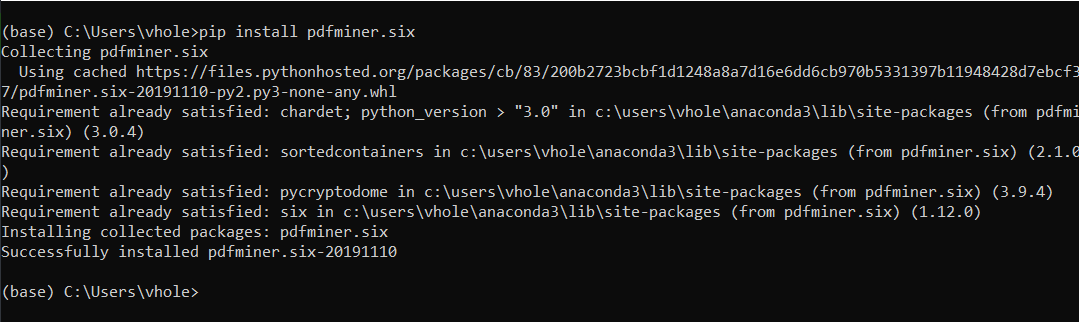
\includegraphics[scale=0.53]{Install_pdfminer_six.PNG}\newline
It has been done successfully when the last thing the prompt says is: "successfully installed pdfminer.six". From here everything we have to do is happening in R. Python is all set up for doing what we want it to do. Now we will work towards using python through RStudio

\subsection{R and RStudio}
R is the program that we have been using during this course and therefore it seems natural to make this script available to be used through R. Making the script usable through R hopefully allows people who are more comfortable in R to use the script as well. To run python in R the package "reticulate" is required. This can be downloaded by running this line in RStudio:
\begin{verbatim}
    install.packages("reticulate")
\end{verbatim}
If this warning is shown, try installing the package Rtools as well: \textit{WARNING: Rtools is required to build R packages but is not currently installed. Please download and install the appropriate version of Rtools before proceeding:} Rtools can be installed like this:
\begin{verbatim}
    install.packages("Rtools")
\end{verbatim}
When reticulate is successfully installed python can be run in R. In my Github repository there is an R-script containing the pieces of code that makes the pdfannots script run in R. The normal console in RStudio is showing a single \textgreater, when running python in R it changes into \textgreater\textgreater\textgreater. To run basic python commands in R we have to use the command:
\begin{verbatim}
    repl_python()
\end{verbatim}
When this is done. The console in R should look like this: \newline
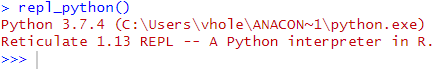
\includegraphics[scale=1]{repl_python.PNG} \newline
Here R tells us, that is ran the command and it has detected python version 3.7.4 in the specified path. When \textgreater\textgreater\textgreater is shown, it means that the console takes python inputs. To return to the console that understands R inputs, simply type in:
\begin{verbatim}
    quit
\end{verbatim}
You have now exited the reticulate python console and are back in the normal R console. This opening and closing of reticulate python is useful to understand how to navigate between Python and R. This command is actually \textbf{not} required when running the pdfannots.py script.This is because the script needs to be run with another command, more on this later.\newline
This was a short description on how to run python in R. If anything is causing trouble, consult the slides of Emma Rand at \url{https://3mmarand.github.io/useR2019_tutorial/#38}

\subsection{Pdfannots.py}
This section of the text will focus on how to install the script, where to put it in your system, how to use it through RStudio and things to remember when working with the script. First things first. We have to have access to the script in order to use it. The script was originally made by Andrew Baumann and it can be found at his Github repository at \url{https://github.com/0xabu/pdfannots}. I have also uploaded the script to my Gitub repository, which can be found here: \url{https://github.com/Digital-Methods-HASS/au590745_Olesen_VictorHarbo/tree/master/pdfannots_in_R/input}, so that it is easy to find both this paper and the script it is about at the same place. All credit for the pdfannots.py script goes to Andrew Baumann. 
\textcolor{red}{Do a part on how i downloaded the script from github and also get my own github working}
\begin{itemize}
\item Implementation details, or the full script demonstrating and documenting all major functions and decisions behind them
\item Empirical Results (product of your script ~slides, map, outline, timeline…)
\end{itemize}{}

\section{Critical evaluation}
\begin{itemize}
\item Comparison with the state-of-the-art software if any (kindly cite relevant work, scripts, etc.)
\item Evaluation of the learning process, time on task, vis-à-vis the product.
\end{itemize}

\section{Conclusions}
Set out the conclusion of this original software publication

\section{Acknowledgements}
Optionally thank people and institutes you need to acknowledge

\section{References}
At least 5 are required
\end{document}
